
\subsection*{Introducció}
\addcontentsline{toc}{subsection}{Introducció}
La comunicació amb llum visible (coneguda com a VLC, acrònim en anglès de "visible light communication") és un mitjà transmissor de dades que utilitza la llum entre 400 i 800 THz (780-375 nm). VLC és un subconjunt de tecnologies de comunicacions òptiques sense fil.



\begin{figure}[h!]
    \centering
    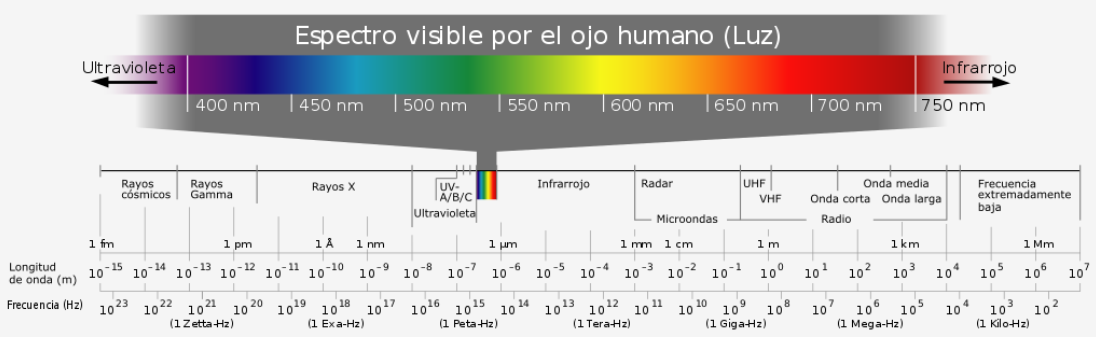
\includegraphics[width=100mm]{llumVisible.png}
    \caption{Espectre del llum visible}
\end{figure}


La tecnologia  VLC utilitza llums fluorescents (làmpades normals, no necessita dispositius especials) per transmetre senyals a una velocitat de 10 kbit/s, o LEDs que pot assolir velocitats de fins a 500 Mbit/s. RONJA (Reasonable Optical Near Joint Access) aconsegueix assolir una velocitat d'Ethernet completa (10 Mbit/s) sobre la mateixa distància gràcies a una òptica més gran i LED més potents.

La VLC pot ser utilitzada com un mitjà transmissor de computació ubiqua, atès que els dispositius que produeixen llum (làmpades d'interior exterior, televisors, senyals de trànsit, lluminosos comercials, fars de vehicles3) utilitzats a tot arreu, es poden aprofitar. El fer ús de la llum visible és també menys perillosa per a aplicacions que utilitzen una gran potència, ja que, els éssers humans poden percebre i protegirse-se del dany que pugui ocasionar-los.



\section*{Tecnologies inalàmbriques}
\addcontentsline{toc}{subsection}{Tecnologies inalàmbriques}

Els subconjunts de tecnologies de comunicació òptiques sense fil són:
\begin{itemize}
    \item Li-Fi: és una nova tecnologia de comunicació sense fils per proporcionar accés a Internet a través de la llum.
    \item Infraroig (IR): Encara que no és visible per a l'ull humà, la llum infraroja s'utilitza en diverses tecnologies sense fil, com ara els controls remots, els dispositius de comunicació a curta distància i les transmissions de dades sense fil en alguns contextos.
    \item Comunicació Òptica d'Espai Lliure (FSO): Aquesta tecnologia utilitza feixos de llum làser per a la transmissió de dades sense cables a través de l'espai lliure, com ara entre dos edificis. És especialment útil en línies de vista directa sense obstruccions.
    \item Comunicació Òptica Inalàmbrica (OWC): Aquesta tecnologia inclou diverses formes de transmissió de dades sense fil a través de llum òptica, incloent l'ús de làsers i LED.
    \item Comunicació Òptica en Entorns Controlats: En alguns entorns, com ara entorns d'oficines o fàbriques, es poden utilitzar sistemes d'òptica sense fil per a la transmissió de dades en lloc de les tecnologies tradicionals sense fil.
\end{itemize}

cada tecnologia té les seves pròpies aplicacions, avantatges i desavantatges. La selecció de la tecnologia òptica sense fil adequada depèn dels requisits específics de l'aplicació i les condicions de l'entorn.

L'estàndard IEEE 802.15.7 estableix les especificacions per a la comunicació sense fils de curt abast utilitzant tecnologies òptiques, com LED i làser. Defineix els protocols i especificacions de capa física i denllaç de dades per a les comunicacions a través de la llum visible.